\documentclass[12pt]{article}
\usepackage[margin = 1in]{geometry}
\usepackage{amsfonts, amsmath, amssymb}
\usepackage[none]{hyphenat}
\usepackage{fancyhdr}
\usepackage{graphicx}
\usepackage{float}
\usepackage[nottoc, notlot, notlof]{tocbibind}
\usepackage{dblfloatfix}
\usepackage{graphicx}

\newtheorem{thm}{Theorem}
\newtheorem{exer}{Exercise}
\newtheorem{lem}[thm]{Lemma}
\newtheorem{defn}{Definition}[section]
\newtheorem{exmp}{Example}[defn]
\newtheorem{prop}[thm]{Proposition}
\newtheorem{cor}{Corollary}[thm]
\newtheorem{conj}{Conjecture}[thm]
\newtheorem{state}{Statement}[thm]
\newtheorem{remk}{Remark}[defn]

%\parindent 0ex
\renewcommand{\baselinestretch}{1.25}

\begin{document}

\begin{titlepage}
\begin{center}
\Large Hello
\end{center}
\end{titlepage}

\tableofcontents
\thispagestyle{empty}
\clearpage

\setcounter{page}{1}

\section*{Summary Sheet}

\newpage

\section*{Memo}

\newpage

\section{Energy Profiles}

\newpage

\subsection{Arizona}

\Large Key Facts:

\normalsize

\begin{itemize}

\item

\item

\item

\end{itemize}

\begin{figure*}[!b]
    \centering
    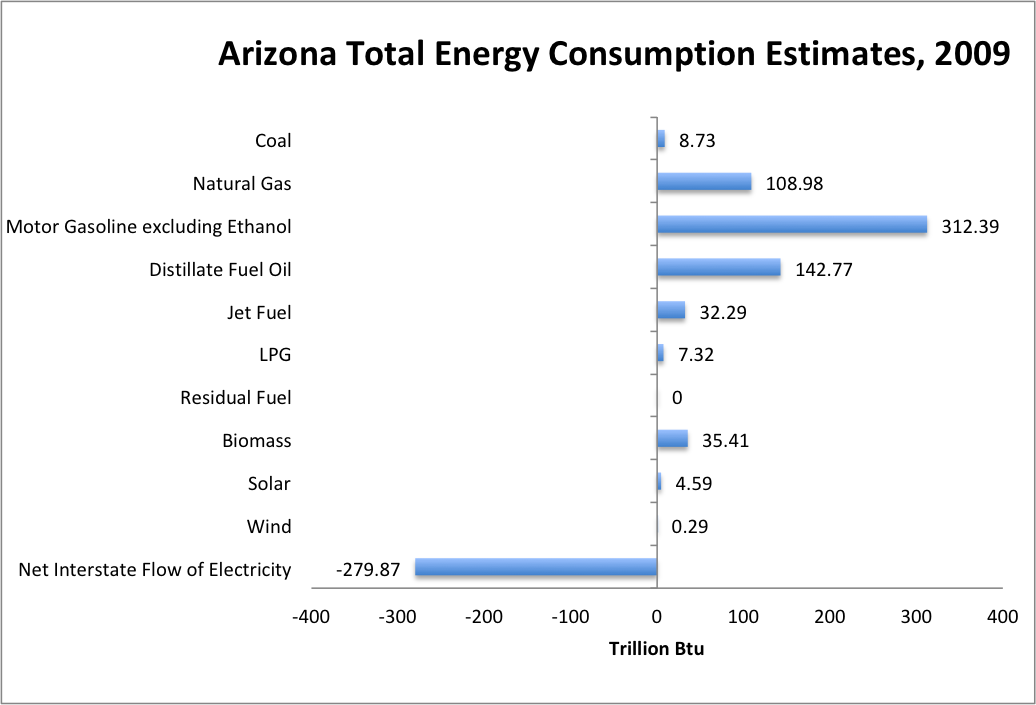
\includegraphics[width=\linewidth]{ArizonaQuickGraph}
\end{figure*}

\newpage

\subsection{California}

\Large Key Facts:

\normalsize

\begin{itemize}

\item

\item

\item

\end{itemize}

\begin{figure*}[!b]
    \centering
    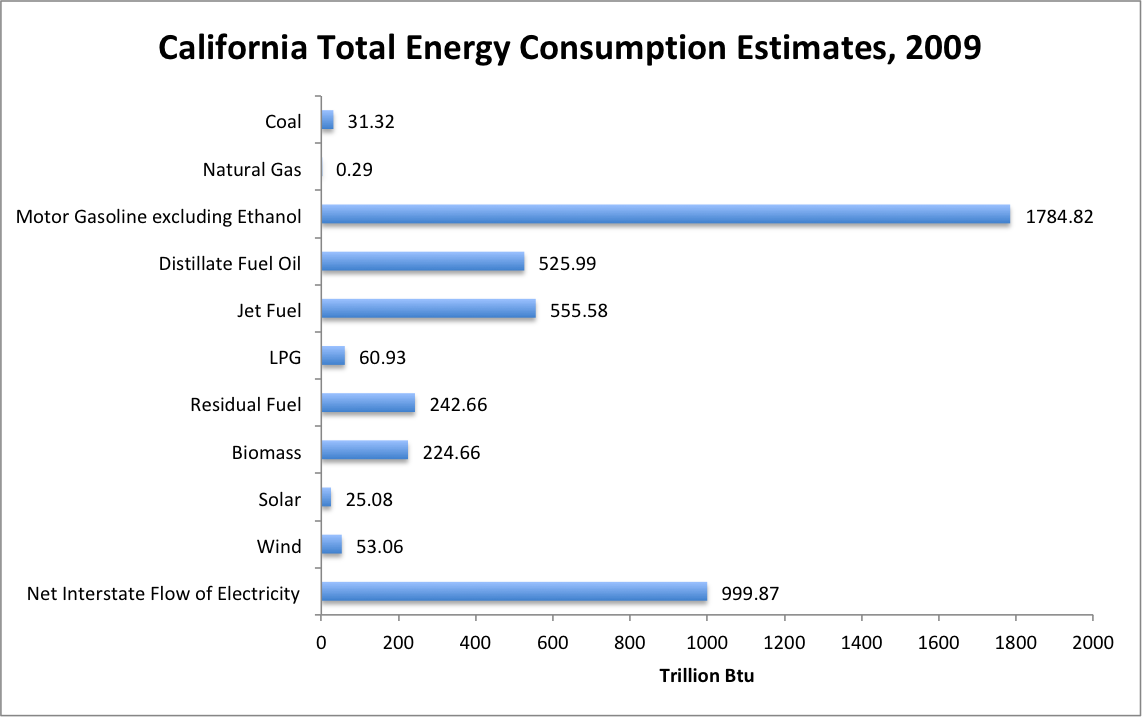
\includegraphics[width=\linewidth]{CaliforniaQuickGraph}
\end{figure*}

\newpage

\subsection{New Mexico}

\Large Key Facts:

\normalsize

\begin{itemize}

\item

\item

\item

\end{itemize}

\begin{figure*}[!b]
    \centering
    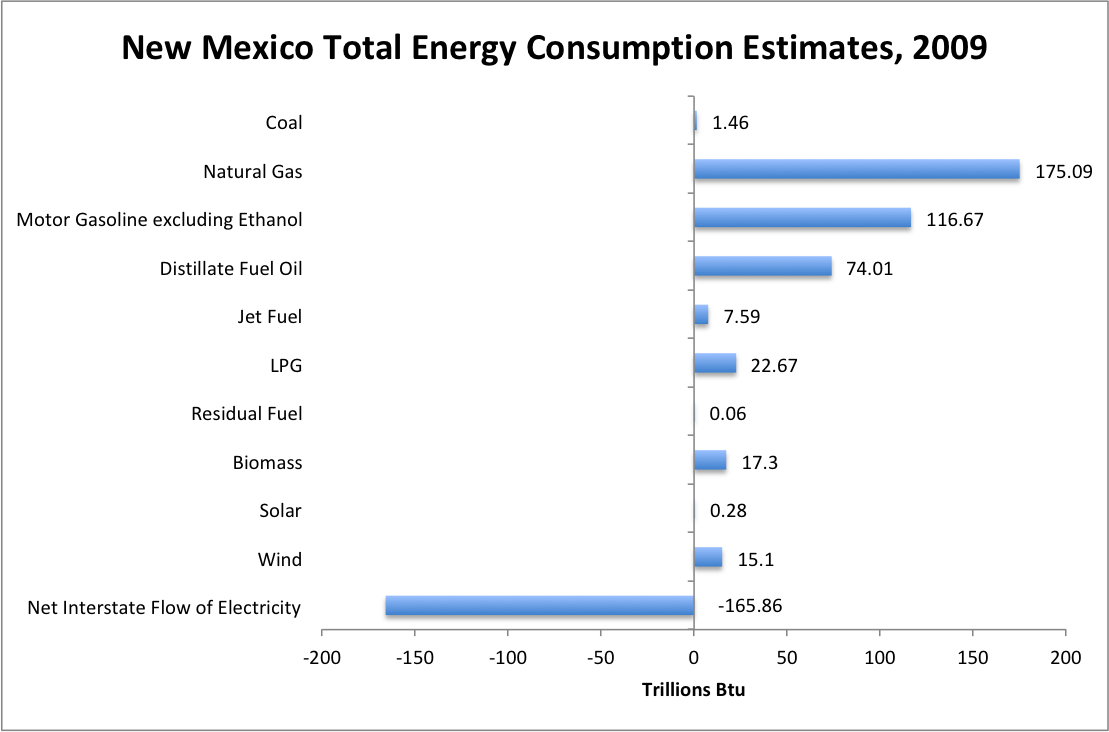
\includegraphics[width=\linewidth]{NewMexicoQuickGraph}
\end{figure*}

\newpage

\subsection{Texas}

\Large Key Facts:

\normalsize

\begin{itemize}

\item

\item

\item

\end{itemize}

\begin{figure*}[!b]
    \centering
    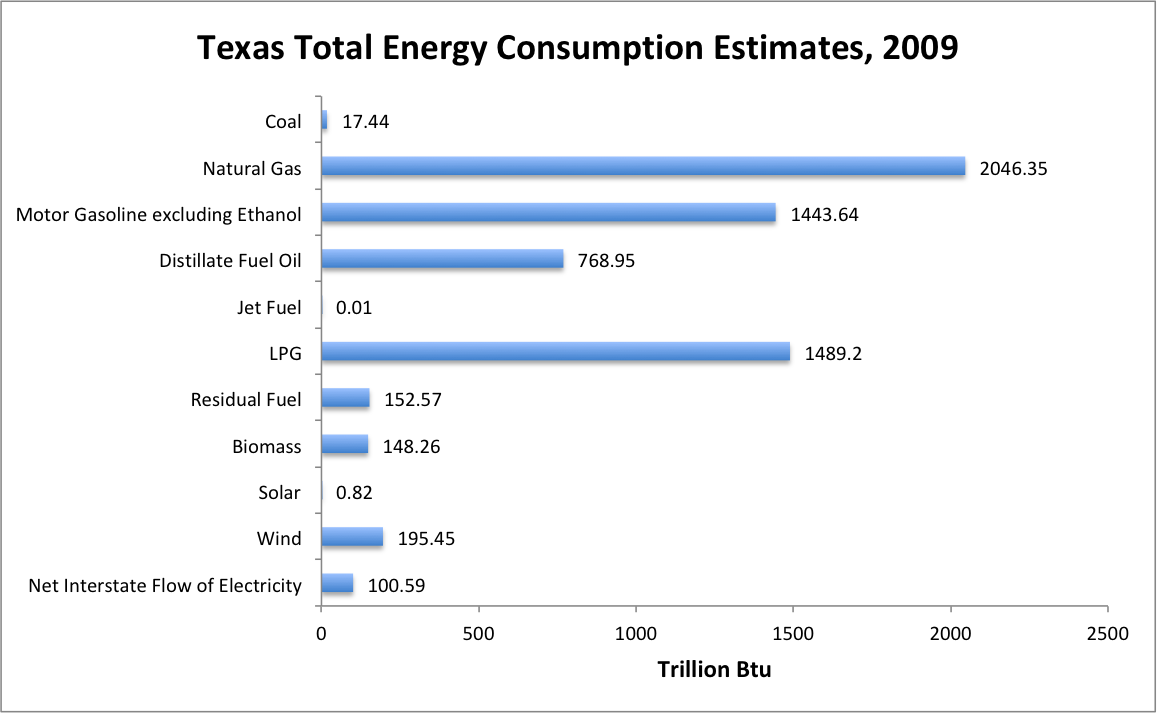
\includegraphics[width=\linewidth]{TexasQuickGraph}
\end{figure*}

\newpage

\begin{thebibliography}{}

\end{thebibliography}


\end{document}
